% !TEX root = ../rapport.tex

\chapter{Conclusion}\label{conclusion}

\section{Bilan de notre travail de groupe}
La diffusion est primordiale dans les réseaux de capteurs sans fils. Dans ce TER, nous avons présenté le problème, puis établi un cadre formel nous permettant de présenter et de simuler quelques algorithmes. Notre travail de groupe a été planifié par le diagramme de GANTT (\ref{GANTT}) que nous avons élaboré.

Nous nous sommes tout d'abord entendus pour que chacun lise deux articles différents afin d'approfondir notre vision d'ensemble du sujet. Puis nous avons constitué 2 sous-groupes : le premier qui commençait la programmation des principaux algorithmes de routage et le second qui approfondissait les recherches. Quelques semaines plus tard, étant satisfaits de l'avancement de la programmation, nous avons décidé de diminuer le nombre de programmeurs et réorienté les ressources sur la rédaction du rapport.

Pour le bon déroulement de notre travail, nous avons utilisé \emph{GIT} et \emph{github} comme moyens de travail collaboratif. Nous avons également organisé des réunions régulières (toutes les une ou deux semaines). Entre ces réunions, nous avons communiqué par mails.


\begin{landscape}
\begin{figure}
\centering
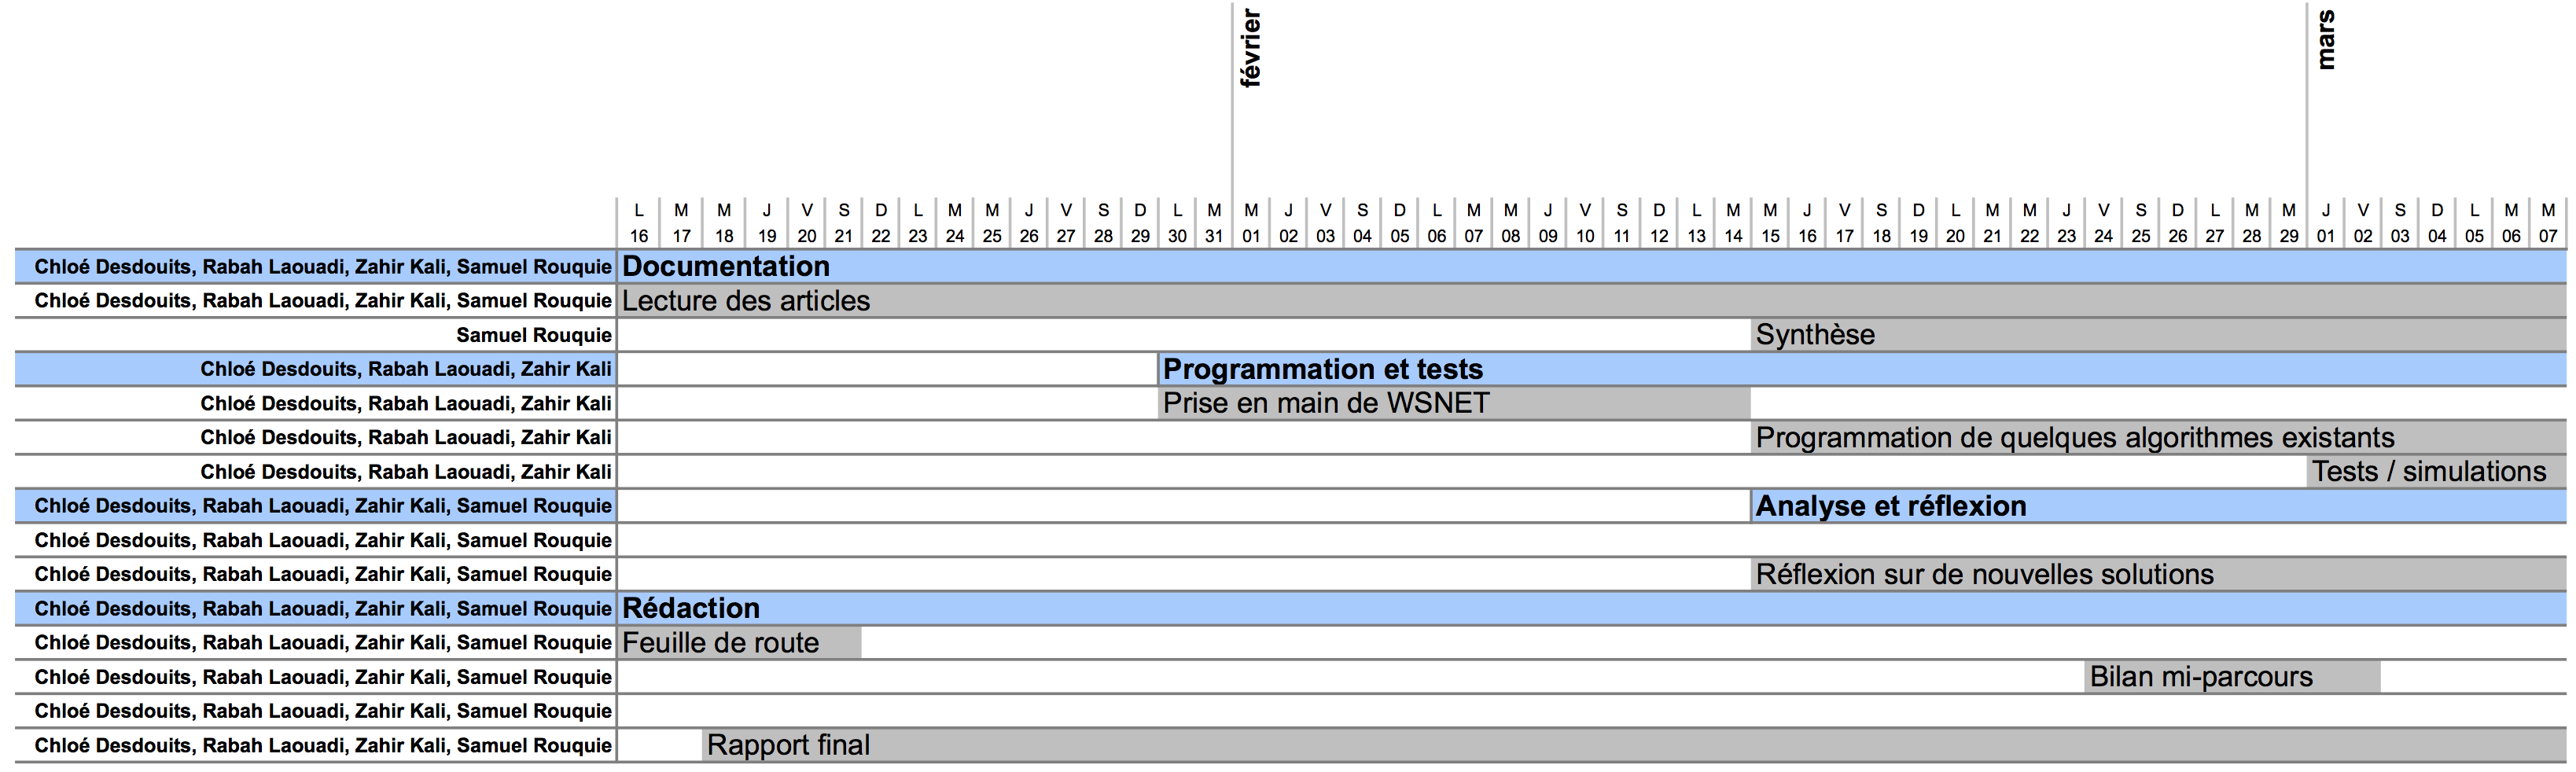
\includegraphics[scale=0.98]{Conclusion/diagramme}
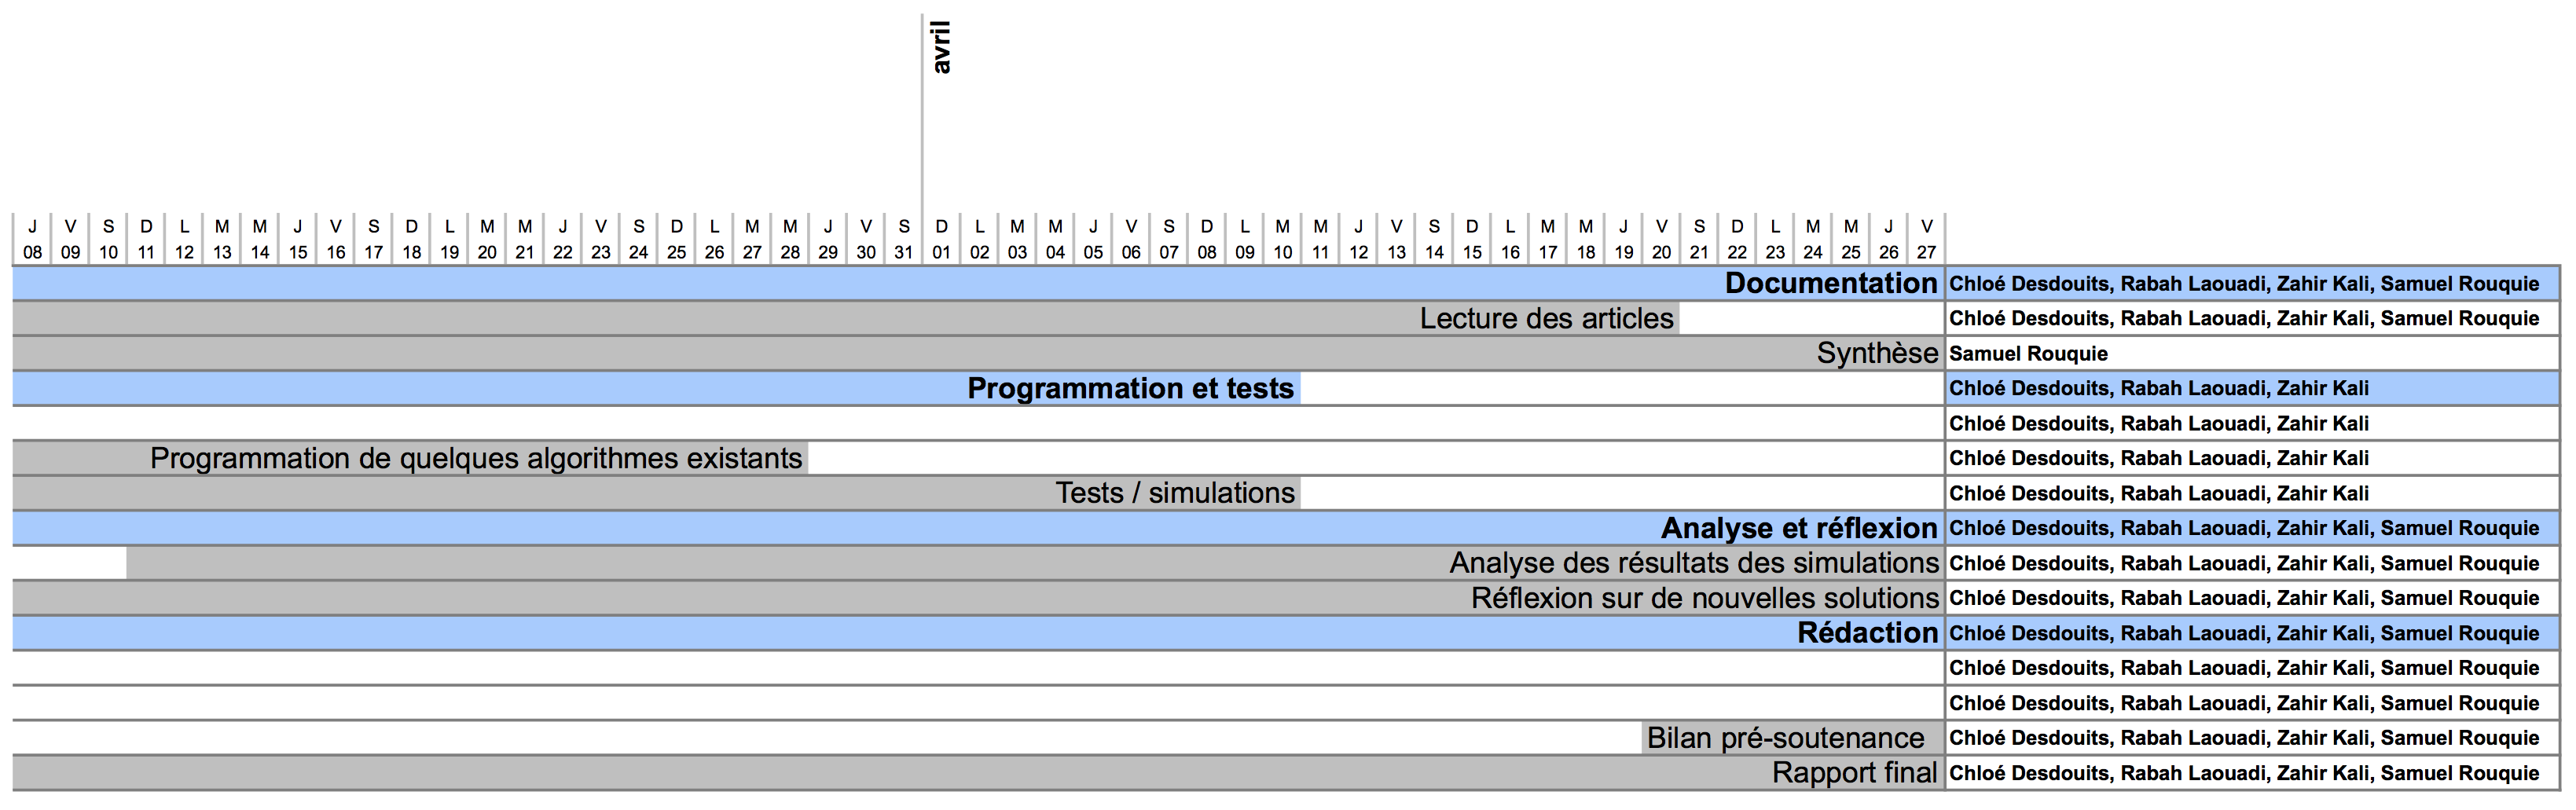
\includegraphics[scale=0.98]{Conclusion/diagramme2}
\label{GANTT}
\end{figure}
\end{landscape}

\section{Bilan du TER}

\subsection{Problèmes rencontrés}
Durant notre travail, nous avons rencontré quelques problèmes dus à l'ambiguité du thème, et ceci particulièrement
dans la désignation des choix des algorithmes qui convergent le plus vers notre sujet. Ceci s'ajoute à la difficulté 
de la prise en main de GIT et de \LaTeX{} puisque la moitié du groupe n'y était pas familiarisé.

\subsection{Contributions}
Dans le cadre de ce TER, nous avons contribué à établir une classification des algorithmes existants. Nous avons également présentés les différents modèles théoriques utilisés et mis en évidence le manque de cohérence des différentes publications. Enfin, nous avons développé différents modules pour WSNET et comparé les performances des principaux algorithmes de routage dans les réseaux de capteurs.





